\section{Additional internal-routing diagnostics}
\label{app:internal_routing}

\paragraph{Evaluation protocol and routing statistics.}
We analyze the frozen circular-cylinder Hopf and Periodic specialists on their held-out autonomous rollout windows.
For the Periodic specialist, we use 13 fixed windows at each of four held-out Reynolds numbers, giving 52 windows of length $K=48$. For the Hopf specialist, we use five fixed windows at each of three held-out Reynolds numbers, giving 15 windows of length $K=56$.One routing record is collected per macro-step at the first integration stage, resulting in 2496 Periodic and 840 Hopf routing decisions per channel. Thus the reported statistics characterize macro-step routing rather than all intermediate right-hand-side evaluations. Overlapping windows are not interpreted as independent trajectories, and these diagnostics are not used for model selection.

For $N$ routing decisions, let $I_{n,e}\in\{0,1\}$ indicate whether routed expert $e$ is selected at decision $n$, with the group identity included in the expert label. We define the normalized activation frequency
\begin{equation}
  f_e
  =
  \frac{1}{2N}
  \sum_{n=1}^{N} I_{n,e},
  \label{eq:app_routing_frequency}
\end{equation}
where the factor $2$ accounts for the Top-2 routed experts selected at each decision, so that $\sum_e f_e=1$. The corresponding mean routing mass is
\begin{equation}
  m_e
  =
  \frac{1}{N}
  \sum_{n=1}^{N}
  \omega_{n,e}I_{n,e},
  \label{eq:app_routing_mass}
\end{equation}
where $\omega_{n,e}$ denotes the final routed mixing coefficient assigned to expert $e$. Experts that are never selected are retained with $f_e=m_e=0$.

We summarize the dispersion of expert selection by the normalized utilization entropy
\begin{equation}
  H
  =
  -\frac{
    \sum_{e:f_e>0} f_e\log f_e
  }{
    \log N_E
  },
  \qquad
  0\le H\le1,
  \label{eq:app_routing_entropy}
\end{equation}
where $N_E$ is the number of routed experts available to the corresponding channel. Because $H$ is computed from activation frequency rather than routing mass, it characterizes diversity of expert selection rather than equality of the assigned weights. Distinct Top-2 pairs retain group identity but are treated as unordered.

For the two specialists considered here, the architecture assigns a fixed coefficient $4/7$ to the shared expert and a total coefficient $3/7$ to the routed Top-2 component. Consequently,
\begin{equation}
  \sum_e m_e=\frac{3}{7}.
\end{equation}
The routing mass therefore measures mixture allocation rather than the norm or physical importance of an expert output.
Labels such as \texttt{g0:e0} refer only to routed experts and should not be confused with the shared expert $e=0$ in
Eq.~(\plaineqref{eq:app_channel_sparse_moe}).

\begin{table}[htbp]
\centering
\caption{
Post-hoc internal-routing statistics for the circular-cylinder Hopf and Periodic specialists on held-out autonomous rollout windows. ``Dominant pair'' denotes the fraction of routing decisions associated with the most frequently selected unordered Top-2 pair.
}
\label{tab:internal_routing_summary}
\small
\setlength{\tabcolsep}{5pt}
\begin{tabular}{@{}llrrrr@{}}
\toprule
Specialist & Channel & Used experts & Distinct pairs & Dominant pair (\%) & $H$ \\
\midrule
Hopf & Velocity & 2/6 & 1 & 100.00 & 0.387 \\
     & Pressure & 2/6 & 1 & 100.00 & 0.387 \\
\addlinespace
Periodic & Velocity & 18/18 & 33 & 16.27 & 0.929 \\
         & Pressure & 14/18 & 16 & 31.25 & 0.784 \\
\bottomrule
\end{tabular}
\end{table}

\paragraph{Periodic routing profile.}
The Periodic specialist uses a broad range of its available routed experts. Across the held-out rollouts, the velocity channel selects all 18 routed experts and realizes 33 distinct group--pair combinations, while the pressure channel selects 14 of 18 experts through 16 combinations (Table~\ref{tab:internal_routing_summary}). The most frequent pair accounts for only $16.27\%$ of velocity decisions and $31.25\%$ of pressure decisions, consistent with the higher utilization entropy of the velocity channel. The selected groups also vary across the four held-out Reynolds numbers.
Figure~\ref{fig:periodic_internal_routing} summarizes the corresponding group frequencies and routed-expert masses.

\begin{figure}[htbp]
\centering
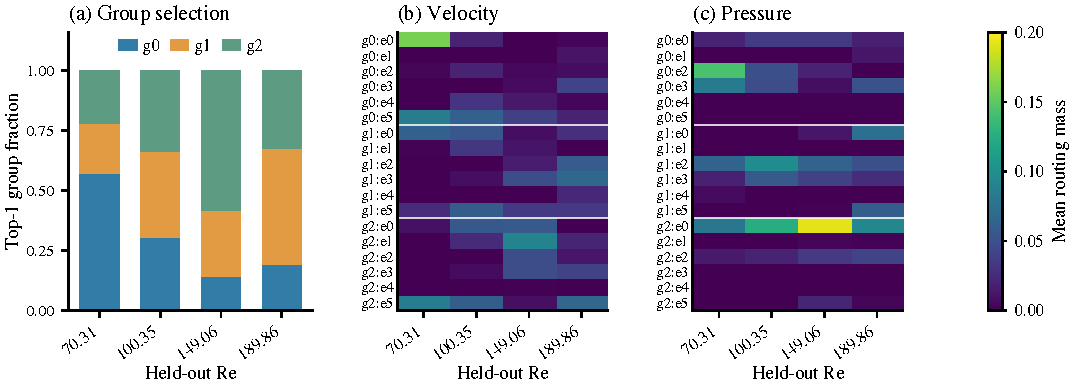
\includegraphics[width=\linewidth]{figures/periodic_internal_routing.pdf}
\caption{
Internal routing of the circular-cylinder Periodic specialist on held-out autonomous rollouts, recorded once per macro-step at the first integration stage. (a) Top-1 group-selection frequencies. (b,c) Mean routed-expert mass for the velocity and pressure channels. Expert identifiers are local to the corresponding specialist, group, and channel and are not assigned physical labels.
}
\label{fig:periodic_internal_routing}
\end{figure}

\paragraph{Hopf routing profile.}
The Hopf specialist exhibits a substantially more concentrated routing pattern. Because it contains a single expert group, only channel-level routing is active. Across all evaluated windows, the velocity channel selects the pair
$(e_1,e_3)$ and the pressure channel selects $(e_2,e_4)$ at every recorded macro-step. A separate stage-wise check confirms that these same pairs are retained across all four Runge--Kutta stages.

Although the selected support is fixed, the routed weights are strongly nonuniform. Velocity expert $e_3$ receives approximately $99.93\%$ of the total routed mass, while pressure expert $e_2$ receives $84.16\%$. The secondary pressure expert $e_4$ nevertheless receives a Reynolds-number-dependent weight, with its mean mass increasing across the three held-out parameter values.

The two specialists therefore exhibit different internal utilization patterns. The Periodic specialist distributes routing decisions across many group--pair combinations, whereas the Hopf specialist retains fixed sparse support and adapts primarily through the mixture weights. The single Hopf group is part of the prescribed architecture and should not be interpreted as collapse of a learned multi-group router.

\paragraph{Periodic rollout-position diagnostic.}
Figure~\ref{fig:periodic_routing_step} shows the mean routed-expert mass as a function of normalized rollout position, using the same 52 held-out Periodic windows. The horizontal coordinate reflects prediction position within the
autonomous window rather than physical oscillation phase. This diagnostic complements the aggregate statistics above by showing how expert allocation varies over the recursive rollout.

\begin{figure}[htbp]
\centering
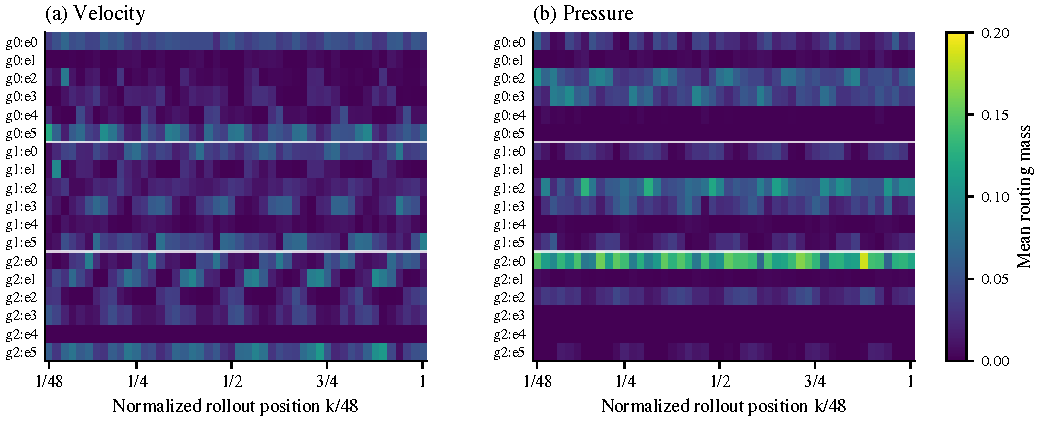
\includegraphics[width=\linewidth]{figures/periodic_rollout_step_routing.pdf}
\caption{
Routed-expert mass versus autonomous rollout position for the circular-cylinder Periodic specialist. Each column averages the routing decision at the corresponding macro-step over the 52 fixed held-out windows, and all routed experts are retained. The horizontal coordinate is the normalized prediction position $k/48$ and is not interpreted as physical oscillation phase.
}
\label{fig:periodic_routing_step}
\end{figure}